\documentclass{report}
% Autor: Roland Bless 1996-2007, bless <at> tm.uka.de
% ----------------------------------------------------------------
% Diplomarbeit - Hauptdokument
% ----------------------------------------------------------------
%%
%% $Id: diplarb.tex 35 2007-01-23 10:56:12Z bless $
%%
% wissdoc Optionen: draft, relaxed, pdf --> siehe wissdoc.cls
% ------------------------------------------------------------------
% Weitere packages: (Dokumentation dazu durch "latex <package>.dtx")
\usepackage{bibgerm}
\usepackage[numbers,sort&compress]{natbib}
\usepackage{amsmath,amssymb,mathtools}
\usepackage{algpseudocode,algorithm}
\usepackage{graphicx}
\usepackage{hyperref}
\usepackage{multirow}
\usepackage[utf8]{inputenc}
\usepackage{geometry}
\geometry{verbose,a4paper,tmargin=25mm,bmargin=25mm,lmargin=15mm,rmargin=20mm}
\DeclareMathOperator*{\argmax}{arg\,max}
\DeclareMathOperator*{\argmin}{arg\,min}

\newcommand{\IndState}[1][1]{\State\hspace{10mm}}
\newcommand{\mparagraph}[1]{\paragraph{#1} \mbox{}\\}

%%%%%%%%%%%%%% includeonly %%%%%%%%%%%%%%%%%%%
% Es werden nur die Teile eingebunden, die hier
% aufgefuehrt sind!
%\includeonly
%%%%%%%%%%%%%%%%%%%%%%%%%%%%%%%%%%%%%%%%%%%%%%
\graphicspath{{pic/}}

\begin{document}
\tableofcontents
\chapter{Allgemein}
\label{chap:Allgemein}

\paragraph{Definition Maschinelles Lernen}

\begin{itemize}
    \item Ein System lernt aus Erfahrung E in Hinblick auf eine Klasse von Aufgaben
    T und einem Performanzmaß P wenn seine Leistung bei Aufgaben aus T gemessen mit
    P durch Erfahrungen aus E steigt
    \item z.B T: Schachspielen, P: Prozent der gewonnen Spiele, E: Spiele gegen sich selbst.
\end{itemize}

\paragraph{Was ist Intelligenz?}
\label{par:Was ist Intelligenz?}
\begin{itemize}
    \item Problemlösung, Erinnern, Sprache, Kreativität, Bewusstsein, Überleben
    in komplexen Welten
\end{itemize}

\paragraph{Wissensrepräsentation}
\label{par:Wissensrepraesentation}
\begin{itemize}
    \item Assoziierte Paare (Eingangs und Ausgangsvariablen)
    \item Parameter in algebraischen Ausdrücken
    \item Entscheidungsbäume
    \item Formale Grammatik
    \item Produktionsregel
    \item Formale logikbasierte Ausdrücke
    \item Graphen und Netzwerke
    \item Probabilistische, graphische Modell
    \item Frames, Schemata, Semantische Netze
    \item Prozedurale Kodierung
    \item Taxonomien
    \item Markov Ketten
\end{itemize}

\begin{figure}[!h]
  \centering
  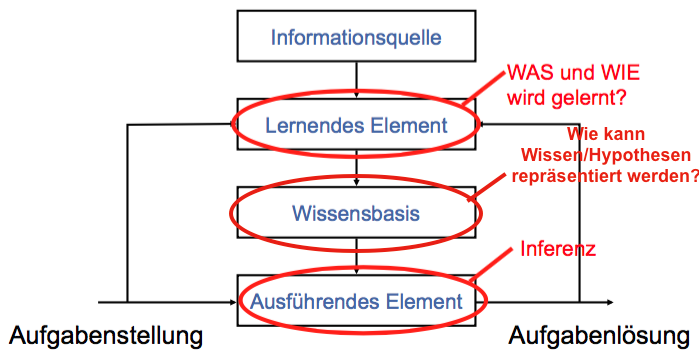
\includegraphics[scale=0.6]{lernendessystem}
  \caption{Komponenten eines Lernenden Systems}
\end{figure}

\paragraph{Inferenz}\mbox{} \\
Vorgang wie ein Programm aus Fakten und Vermutungen (''Korrekte'') Schlüsse
ziehen kann. \\
Aus einer Menge von Formeln A folgt B $\Leftrightarrow$ Es gibt eine Folge von Regeln
um B abzuleiten

\paragraph{Modus Ponens}\mbox{} \\
%$\frac{\text{A, A\rightarrow B}}{\text{B}}$
 Besagt, dass wenn A $\rightarrow$ B und A gilt,
dann gilt auch B. $\frac{A, A \rightarrow B}{B}$

\paragraph{Abduktion} \mbox{} \\
Deduktion beweist, dass etwas ist. Induktion zeigt dass etwas anwendbar ist.
Abduktion zeigt nur, dass etwas sein kann
\begin{enumerate}
    \item alle Menschen sind sterblich
    \item Sokrates ist Mensch
    \item Sokrates ist sterblich
\end{enumerate}

\chapter{Induktives Lernen}
Eine große Menge an Beispielen wird gegeben. Der Lerner muss selbst das Konzept herausfinden.

\paragraph{Version Space} \mbox{} \\
Der Raum aller Hypothesen, welche mit den Trainigsbeispielen konsistent sind.

\paragraph{Konzept} \mbox{} \\
Ein Konzept beschreibt Untermenge von Objekten oder Ereignissen definiert auf
einer größeren Menge

\paragraph{Konsistenz} \mbox{} \\
Keine negativen Beispiele werden positiv klassifiziert.

\paragraph{Vollständigkeit} \mbox{} \\
Alle positiven Beispiele werden als positiv klassifiziert.

\paragraph{Lernen als Suche im Hypothesenraum} \mbox{}
\begin{itemize}
    \item \textbf{Algorithmen}
    \begin{itemize}
        \item Suche vom Allgemeinen zum Speziellen: Negative Beispiele führen zur
        Spezialisierung
        \item Suche vom Speziellen zum Allgemeinen: Positive Beispiele führen zur
        Verallgemeinerung
        \item Version Space: Paralleles Verwenden der oben genannten Anwendungen.
    \end{itemize}
    \item \textbf{Präzedensgraph}
    \begin{itemize}
        \item In welcher Reihenfolge werden Aktionen ausgeführt?
        \item Codierung der Hypothese mit Gerichtetem, azyklischem Graphen
    \end{itemize}
\end{itemize}

\paragraph{Version Space Algorithmus} \mbox{} \\
Der Version Space Algorithmus ist ein binärer Klassifikator für diskrete
Feature-Spaces.
\begin{itemize}
    \item Beginne mit generellster Hypothese $G=(?,...,?)$ und speziellester
    Hypothese $S = (\#,...,\#)$
    \item Ist Beispiel false
    \begin{itemize}
        \item Lösche aus S Hypothesen, die Beispiel abdecken
        \item Spezialisiere Hypothesen in G soweit, dass sie das Beispiel nicht abdecken
        und allgemeiner als eine Hypothese in S bleiben.
        \item Lösche aus G alle Hypothesen, die spezifischer als eine andere
        Hypothese in G sind
        \item Kurz: spezialisiere generellste Hypothese
    \end{itemize}
    \item Ist Beispiel true
    \begin{itemize}
        \item Lösche aus G Hypothesen, die mit Beispiel inkonsistenten Hypothesen
        \item Verallgemeinere die Hypothesen in S soweit, dass sie Beispiel abdecken
        und dass sie spezifischer als eine Hypothese in G bleiben
        \item Lösche aus S alle Hypothesen, die allgemeiner als eine andere
        Hypothese aus S sind
        \item Kurz: Passe speziellste Hypothese an und verallgemeinere
    \end{itemize}
    So kann man den Raum aller mit den Trainigsdaten konsistenten Hypothesen
    finden.

    \item Positive Aspekte
    \begin{itemize}
        \item feststellbar, welche Art von Beispiele noch nötig ist
        \item feststellbar, wann das Lernen abgeschlossen ist
    \end{itemize}
\end{itemize}
\paragraph{Induktiver Bias} \mbox{} \\
Induktives Lernen erfordert Vorannahmen. Bias ist die Vorschrift, nach der Hypothesen
gebildet werden.

\chapter{Reinforcement Learning}
Lernen durch Belohnung \\
\textbf{Lernziel:} Finde Aktionssequenz $a_1, a_2, ...,a_n$, sodass dadurch die
maximale Bewertung aufgesammelt wird

\paragraph{Markrow-Entscheidungsproblem (Markrov Decision Process, MDP)} \mbox{}\\

Ein MDP ist ein 5-Tupel $(S, A, P, R, \gamma)$ wobei
\begin{itemize}
    \item $S$: Endliche Zustandsmenge (States), ''Sensorik''
    \item $A(s)$: Menge möglicher Aktionen im Zustand $s$, ''Aktorik''
    \item Zustandsänderung (meist bekannt oder beobachtbar )\\
    $\delta: (S \times A) \rightarrow S$\\ $\delta(s_t,a_t) = s_{t+1}$\\
    Markov Bedingung: keine Abhängigkeit von der Vergangenheit
    \item Bewertung von Aktionen (direkt oder indirekt messbar/bekannt)\\
    $r:(S \times A) \rightarrow R \\ r(s_t,a_t) = r_t \\$
    Die direkte Belohnung wenn durch Aktion a im Zustand s ausgeführt wurde
    \item $\gamma \in [0,1]$ Diskontierungsfaktor, zeigt Bedeutung von direkter
    Belohnung im Vergleich zu zukünfitger Belohnung an.
    \begin{itemize}
        \item $\gamma = 0$: aktuelle Aktionsbewertung ist wichtig (1-Step)
        \item $\gamma > 0$: zukünftige (letzte) Bewertungen werden berücksichtigt. (n-step)
        \item $\gamma < 1$: Notwendig um konvergente V-Funktionen (Value function) zu erhalten.
    \end{itemize}
\end{itemize}

\section{Reinforcement Learning}
Beim RL liegt ein MDP vor. Es gibt also einen Agenten, der Aktionen ausführen kann.
Diese können (nicht notwendigerweise) sofort bewerten werden.

\paragraph{Policy} \mbox{} \\
Policy ist eine Vorschrift $\pi: S \rightarrow A$, in welchem Zustand welche Aktion
ausgeführt werden soll.
\paragraph{Policy Learning} \mbox{} \\
Gesucht $S_{1} \xrightarrow[a_1]{r_1}S_{2}\xrightarrow[a_2]{r_2}\dots \xrightarrow[a_{n-1}]{r_{n-1}}S_n$
Finde optimale Policy $\pi^{*}$
\paragraph{Value Function} \mbox{} \\
Die Funktion $V^{\pi}:S\rightarrow \mathbb{R}$ gibt den erwarteten Wert (nicht Belohnung, da $\gamma$ eingeht)
eines Zustand $s$ unter der policy $\pi$ an. Mit $V^{*}$ wird der Wert unter der
optimalen policy bezeichnet. \\
$V^{\pi}(s_t) = r_t + {\gamma} r_{t+1} + {\gamma}^2 r_{t_2} + \dots = \sum\limits_{i=0}^{\infty} \gamma^i r_{t+1}$
\begin{itemize}
    \item optimale Zielfunktion: $\pi^{*}(s) = \underset{\pi}{\mathrm{argmax}} V^{\pi}, \forall s$
    \item max. akkumulierte Bewertung: $V^{*} = V^{\pi^{*}}(s)$
    \item rekursive Definition (Bellman Gl.): $V^{*}(s_t) = r_t + \gamma V^{*}(s_{t+1})$
\end{itemize}

\paragraph{Simple Value Iteration} \mbox{} \\
\begin{algorithm}[H]
    \begin{algorithmic}
        \State Initialisiere $\hat{V^{*}}(s)$ zufällig
        \While{} forever
            \State wähle einen Zustand $S_t$
            \State ermittle beste Aktion und den Folgezustand
            \State $s_t = \delta(s_t,\pi^{*}(s_t)))$
            \State ersetzte
            \State $V^{*}(s_t) = r_t + \gamma V^{*}(s_{t+1})$
            \EndWhile
    \caption{Value Iteration}
    \end{algorithmic}
\end{algorithm}

Simple Value Iteration schätzt die Value Function ab, indem sie solange wie nötig
aktualisiert wird bis sie konvergiert.

\paragraph{Simple Temporal Difference Learning} \mbox{} \\
Funktioniert genau wie Simple Value Iteration, nur dass die
Value Function mit einer learning rate $\alpha$ aktualisiert wird:\\
\begin{itemize}
    \item $\hat{V}^{*}(s_t) = (1-\alpha) * \hat{V}^{*}(s_t)+\alpha(r_t + \gamma \hat{V}^{*}(s_{t+1}))$
\end{itemize}
\paragraph{Q-Funktion} \mbox{} \\
Die Funktion $Q : S \times A \rightarrow \mathbb{R}$, $Q(s,a)$ gibt die maximale
Bewertung, die erreicht werden kann im Zustand $s$ durch die Aktion $a$.
\paragraph{Q-Learning} \mbox{} \\
\begin{algorithm}
\begin{algorithmic}
    \State Ziel: Finde Schätzung $\hat{Q}(s,a)$ der absoluten Funktion $Q(s,a)$
    \State Lernen
    \State Initialisiere $\forall s,a$ $\hat{Q}(s,a) = 0$
    \State Wähle Zustand
    \While{} Forever:
        \State wähle Aktion $a$ und führe aus
        \State $r \leftarrow$ direkte Bewertung (reward)
        \State neuer Zustand $s'$
        \State update
        \IndState $\hat{Q}(s,a) \leftarrow r + \gamma \max_{a'} \hat{Q}(s',a')$
        \State $s\leftarrow s'$
        \EndWhile
    \caption{Q-Learning}
\end{algorithmic}

\end{algorithm}

\paragraph{Temporal Difference Learning}\mbox {} \\
Die Differenz folgender Schätzungen als Lernsignal für $\hat{Q}(s,a), \hat{V}^{*}(S)$

Zum predicten nutzt TD die Annahme, dass aufeinander folgende Vorhersagen
oftmals in gewissen Maßen zusammenhängen. Schätzungen werden anhand anderer
gerlernter Schätzungen angepasst ohne auf das Endgültige Ergebniss zu warten.

\mparagraph{Vorwärtssicht (theoretisch)}
\begin{itemize}
    \item Gewichtete Anpassung an direkt nachfolgender Schätzung (1-Step) oder
    \item Gewichtete Anpassung an n Schritte nachfolgender Schätzung (n-step)
\end{itemize}

\mparagraph{Rückwärtssicht}
Fehlersignale (temporal differences) in den Schätzungen werden nach hinten
weitergegeben.

\paragraph{Eligibility Traces, Verantwortlichkeitsspuren} \mbox{} \\
Eligibility Traces sind ein Grundmechanismus des Reinforcment Learning. \\
Es gibt 2 Arten diese zu betrachten:
\begin{itemize}
    \item Die theoretische Weise, dass sie die Brücke von Temporal Difference
    zur Monte Carlo Methode sind (Vorwärtssicht)
    \item Oder, dass eligiblity traces eine Art temporäre Aufnahme eines
    Geschehens in einem Event sind (z.B das Erreichen eines Zustandes oder das
    Ausführen einer Aktion (Rückwärtssicht). Eligibility Traces bietet also ein
    Kurzzeitgedächnis von vielen vorheriger Inputs so dass neue Beobachtungen
    in Bezug auf diese Signale aktualisiert werde können.
\end{itemize}
Die Verwendung von Eligibility Traces wird durch $(\lambda)$ gekennzeichnet (z.B
$TD(\lambda)$)
\paragraph{SARSA} \mbox{} \\
Ist ein Lernalgorithmus, der die Q-Funktion updated:
$Q(s_t,a_t) \leftarrow (1-\alpha) \cdot Q(s_t,a_t) + \alpha [r_{t+1} + \gamma Q(s_{t+1}, a_{t+1})]$

\chapter{Lerntheorie}

\mparagraph{Rasiermesser Prinzip}
Löse nie ein Problem komplizierter als nötig, denn die einfachste, richtige Erklärung
ist die Beste.\\
Von mehreren möglichen Erklärungen für ein und denselben Sachverhalt ist die einfachste
Theorie allen anderen vorzuziehen. Eine Theorie ist einfach, wenn sie möglichst
wenige Variablen und Hypothesen enthält und wenn diese in klaren logischen
Beziehungen zueinander stehen, aus denen der zu erklärende Sachverhalt logisch folgt.

\mparagraph{Definition Lernmaschine}
\begin{itemize}
    \item Eine lernende Maschine wird bestimmt durch:
    \begin{itemize}
        \item Hypothesenraum ${h_\alpha : \alpha \in A}$
        \item Lernverfahren: die Methode um $\alpha_{opt}$ mit Hilfe von
        Lernbeispielen zu finden
    \end{itemize}
    \item Das resultierende Entscheidungsmodell $M_{opt}$. Es ist gegeben durch die Auswertung
    der optimalen Hypothese $h_{opt}$, die durch die lernende(n) Maschine(n) bestimmt wird
\end{itemize}

\mparagraph{Probleme}

\begin{itemize}
    \item \textbf{Statistisches Problem}: Das Verfahren betrachtet einen -
    gemessen an der Menge der Trainigsdaten - ''zu grossen'' Hypothesenraum
    \item \textbf{Komplexitätsproblem}: Aufgrund der Komplexität des Problems kann
    das Lernverfahren nicht das Finden einer optimalen Lösung innerhalb des
    Hypothesenraum garantieren.
    \item \textbf{Repräsentationsproblem}: Der Hypothesenraum enthält keine ausreichend
    gute Approximation der Zielfunktion/Konzept etc.
\end{itemize}

\mparagraph{Overfitting}
Die Tendenz der Maschine sich beim Lernen auf die Lernbeispiele zu spezialisieren
(Auswendig lernen). $\rightarrow$ Lernfehler fällt, Testfehler steigt, Generalisierung fällt.\\

\textbf{Lösung}
\begin{itemize}
    \item Repräsentative Beispiele
    \item Lernprozess durch den Verifikationsfehler steuern.
    \item Richtige Wahl und Suche der optimalen Hypothese $h_a$
\end{itemize}


\mparagraph{Validierung}
\begin{itemize}
    \item Crossvalidation
    \begin{itemize}
        \item Teile Daten in Lern und Validierungsdaten
        \item Bestimmte darauf verschiedene Hypothesen (bzw. deren Parameter)
        \item Berechne jeweils Generalisierung
        \item wiederhole
    \end{itemize}
    \item n-fold-crossvalidation
    \begin{itemize}
        \item Zerlege Daten in n-Mengen
        \item Trainiere auf n-1 Mengen, Teste auf 1 Menge
        \item Wiederhole
    \end{itemize}
    \item Leave One Out
    \begin{itemize}
        \item Jeweils ein Beispiel für das Lernen weglassen
        \item Addiere Fehler für weggelassene Beispiele
        \item Wiederhole
    \end{itemize}
\end{itemize}

\mparagraph{Boosting}
Kombiniere mehrere schwache Modelle um ein gutes zu bekommen, indem Trainigsbeispiele unterschiedlich
gewichtet werden.
\mparagraph{Bagging (Bootstrap aggregating)}
Kombiniere mehrere schwache Modelle um eine gutes zu bekommen. Dabei bekommt jedes
schwache Modell nur eine Teilmenge der Trainigsdaten

\mparagraph{AdaBoost (Adaptive Boosting)}
Lerne einen Klassifikator für die Daten. Finde die fehlerhaft klassifizierten Beispiele
, erhöhe deren Gewichte und trainieren einen neuen Klassifikator, welcher darauf achtet
die höher gewichteten Beispiele richtig zu klassifizieren

\begin{algorithm}[H]
    \begin{algorithmic}
        \State Begin: $D = {(\vec{x}_1,y_1),\dots,(\vec{x}_n,y_n)}$, $W_1(i) = \frac{1}{n}$ (Gewicht pro Beispiel)
        \For {k=1 till $k_{max}$}
        \State Trainiere $M_k$ auf $D_k$ (Anzahl $D_k = n$, Bsp. gewählt ab. von $W_k(i)$)
        \State $E_k \leftarrow$ emp. Fehler von $M_k$ (gewichtet bez. $W_k(i)$) )
        \State $\alpha_k \leftarrow \frac{1}{2} \log \frac{1-E_k}{E_k}$
        \begin{equation}W_{k+1}(i) \leftarrow \frac{W_k(i)}{Z_k}\begin{cases}
            e^{-\alpha_k}, \text{ wenn } h_k(\vec{x}_i) = y_i \\
                                                            e^{\alpha_k}, \text{wenn } h_k(\vec{x}_i) \neq y_i
                                                        \end{cases}\end{equation}
        \EndFor
        \caption{AdaBoost}
    \end{algorithmic}
\end{algorithm}

\mparagraph{Kaskadierung}
Verwende eine Kaskade an Entscheidungen anstatt kombinierter Gewichte.
Ermöglicht das effiziente Filtern und erkennen von richtigen Beispielen.
Dafür werden mehrere Schichten verwendet, wobei die Komplexität mit zunehmender
Schicht steigt. Findet eine Schicht ein negatives Beispiel stoppt die Bearbeitung
dieses Beispielt. Die nächste Schicht versucht nun fälschlicherweise korrekt
erkannte Beispiele (false postive) weiter zu filtern usw.


\mparagraph{Probably approximately correct learning (PAC)}
PAC macht eine Aussage über die anzahl der benötigten Stichproben, wenn
man einen bestimmten realen Fehler mit einer frei zu wählenden Wahrscheinlichkeit
bekommen will.\\\\

Gegeben
\begin{itemize}
    \item Eine Menge $X$ von Instanzen der Länge $n$
    \item ein Konzept $C$
    \item Ein Hypothesenraum $H$
    \item eine Lerndatenmenge $D$
\end{itemize}
Es kann nun mit einer beliebigen Wahrscheinlichkeit $1-\delta, 0<\delta<\frac{1}{2}$ \\
eine $\epsilon$ - genaue Hypothese gefunden werden. $E_d(h) \leq \epsilon, 0<\epsilon<\frac{1}{2}$

Die Anzahl der benötigten Lerndaten ist: \\
$m \geq \frac{1}{\epsilon}(\ln\frac{1}{\delta}+\ln|H|)$ \\
$\Rightarrow$ je größer die gewünschte Sicherheit, je kleiner der zulässige fehler, je größer
der Hypothesenraum, desto größer die Anzahl der benötigten Daten.

\mparagraph{Vapnik-Chervonenkis Dimension}
Die VC Dimension $VC(h_a)$ von $H^\alpha$ ist gleich der maximalen Anzahl von Datenpunkten
(aus einer Menge $S$) die von $H^\alpha$ beliebig separiert werden können.
Eien Abbildung (Hypothese) $h$ separiert die Daten aus $S$ wenn durch $h$ zwei Untermengen
definiert werden:
$\{x|h(x) = 0\} \text{ und } \{x|h(x) = 1\}$

\mparagraph{Structural Risc Minimization, SRM}
SRM ist die Abwägung zwischen einem einfachen Modell und einem komplexen Modell,
welches auf den Trainingsdaten besser funktioniert, aber eventuell mehr unter
Overfitting leidet.
Minimiere den unten genannten Term.

\mparagraph{Abschätzen des realen Fehlers}
Der reale Fehler kann durch den empirischen Fehler und die VC-Dimension wie
folgt abgeschätzt werden:

Mit Wahrscheinlichkeit $P(1-\eta)$ gilt:
\begin{displaymath}
        E(h_\alpha) \leq E_{emp}(h_\alpha) + \sqrt{\frac{VC(h_\alpha)}{N} \cdot (\log(2 N / VC(h_\alpha)) + 1) - \frac{\log(\eta  / 4)}{N}}
\end{displaymath}


wobei gilt:

\begin{itemize}
    \item $E(h_\alpha)$ ist der reale Fehler der mit der Hypothese $h_\alpha$
        gemacht wird
    \item $E_{emp}(h_\alpha)$ ist der empirische Fehler der mit der Hypothese $h_\alpha$
        gemacht wird
    \item $VC(h_\alpha)$ ist die VC-Dimension der Lernmaschine
    \item N ist die Anzahl der Lernbeispiele
    \item $0 \leq \eta \leq 1$
\end{itemize}
Dieser Term wird in der Structural Risc Minimization minimiert.

\chapter{Neuronale Netze}

\mparagraph{Einsatzfelder}
\begin{itemize}
    \item Klassfikation und Mustererkennung (Sprach und Schrifterkennung)
    \item Funktionsapproximation
    \item Mustervervollständigung (Kodierung, Bilderkennung)
\end{itemize}

\mparagraph{Perzeptron nach Rosenblatt}
\begin{itemize}
    \item Auswertung: Input Vektor und Bias mit Gewichten multiplizieren,
    addieren und Aktivierungsfunktion anwenden
    \item Training: Zufällige Initialisierung des Gewichtsvektors, addieren
    von fehlklassifizierten Vektoren auf Gewichtsvektor
\end{itemize}

\mparagraph{Delta Regel}
Lernalgorithmus für Neuronale Netze mit einer Schicht. Ist ein Spezialfall
des allgemeineren Backpropagation Algorithmus.
\begin{equation}
    \Delta w_{ij} \in \alpha(t_j - y_j) \phi'(h_j)x_i
\end{equation}
\begin{itemize}
    \item $\Delta w_{ij} \in \mathbb{R}$ ist die Änderung des Gewichts von Input
    $i$ zum Neuron $j$
    \item $\alpha \in [0,1]$ ist die Lernrate (typischerweise $\alpha$ ca. 0.1)
    \item $ t_j \in \mathbb{R}$ ist der Zielwert des Neurons $j$
    \item $y_j \in \mathbb{R}$ ist die Tatsächliche ausgabe
    \item $\phi'$ ist die ableitung der Aktivierungsfunktion des Neurons
    \item $h_j \in \mathbb{R}$ ist die gewichtete Summe der Eingaben des Neurons
    \item $x_i \in \mathbb{R}$ der $i$-te Input
\end{itemize}
\mparagraph{Gradientenabstieg}
Optimierungsalgorithmus für Differenzierbare Funktionen. Starte an einer zufälligen
Stelle $x_0$ und führe folgenden Schritt mehrfach durch
\begin{equation}
    x_0 \leftarrow x_0 - \alpha(\text{grad})f(x_0)
\end{equation}
\begin{itemize}
    \item $\alpha \in (0,1]$ Lernrate
    \item $f$ ist die zu optimierende Funktion
\end{itemize}
\mparagraph{Backpropagation}
Auf Multilayer Perceptron angepasster Gradientenabstieg.

Initialisiere Gewichte mit kleinen zufälligen Werten.\\

Wiederhole:
\begin{itemize}
    \item Auswahl eines Beispielmusters $d$
    \item Bestimmen der Netzausgabe
    \item Bestimmen des Ausgabefehler (bzgl. Sollausgabe)
    \item Sukzessives Rückpropagieren des Fehlers auf die einzelnen Neuronen
    \item Anpassung der Gewichtsbelegung nach Delta Regel bis Abbruchkriterium
    erfüllt ist.
\end{itemize}

\mparagraph{Radiale Basisfunktion (Radial Basic Function, RBF)}
Eine radiale Basisfunktion ist eine Funktion $f: D \rightarrow \mathbb{R}$,
für die $f(x) = f(\|x\|)$ gilt bzw. allgemeiner, für die ein $c \in D$
existiert, sodass $f(x, c) = f(\|x - c\|)$ gilt. 

Der Wert der Funktion hängt also nur von der Distanz zum Ursprung bzw.
allgemeiner zu einem Punkt $c \in D$ ab.

Ein typisches Beispiel sind gaußsche RBFs:
$f(x) = e^{-(a (x - c)^2)}$, wobei $a, c$ Konstanten sind.

Radial Basis Funktion Netz besteht typischerweise aus einem vorwärtsgerichtetem Netz
mit 3 Schichten (1 Hidden Layer). Die Aktivierungsfunktion ist eine RBF. Jedes Neuron
besitzt zwei Parameter. Radius und Zentrum.

\mparagraph{Resiliant Propagation, RPROP}
RPROP ist ein iteratives Verfahren zur Bestimmung des Minimums der
Fehlerfunktion in einem neuronalen Netz bzw. eine Gewichtsupdate-Regel
für neuronale Netze. Sie betrachtet nur das Vorzeichen des Gradienten,
jedoch nicht den Betrag. Jedes Gewicht wird unabhängig von den anderen behandelt.\\

Fehlerfunktion
\begin{displaymath}
    E = \frac{1}{2} \sum_{i in \text{outputs}}(t_i -o_i)^2
\Delta w_{ij}(t)= \begin{cases}
-\Delta_{ij}(t), \text{ wenn } \frac{\partial E}{\partial w_{ij}}(t) > 0 \\
+\Delta_{ij}(t), \text{ wenn }\frac{\partial E}{\partial w_{ij}}(t) < 0 \\
0, \text{ sonst}
\end{cases}
\end{displaymath}


Der Algorithmus hat Konstanten $\eta^- \in \mathbb{R}_{\le 1}$ sowie
$\eta^+ \in \mathbb{R}_{\ge 1}$. Für jedes Gewicht ist außerdem
$\eta=1$ zu Beginn. Bei jedem Gewichtsupdate wird überprüft, ob sich das Vorzeichen des
Gradienten für dieses Gewicht geändert hat. Falls ja, wird das Gewicht
um $\eta \cdot \eta^+$ bzw $\eta \cdot \eta^-$ geändert. Außerdem
kann eine minimale bzw. eine Maximale Änderung gesetzt werden.


\mparagraph{Cascade Correlation}
Konstruktiver Lernalgorithmus für MLNN.

\begin{enumerate}
    \item Initialisierung: 2-schichtiges Netz, Abruchkriterien: Fehlerschranke,
    Anzahl Neuronen, etc.
    \item Trainieren - Anpassen aller Gewichte
    \item Solange es zu keiner Besserung kommt:
    \begin{itemize}
        \item Füge neues Neuron (Kandidat Neuron) in neue Hiddenschicht und verbinde
        es mit allen Input und output Neuronen.
        \item Trainiere neues Neuron einmalig
        \item Trainiere Netz
    \end{itemize}
\end{enumerate}

\begin{itemize}
    \item zu jedem Zeitpunkt nur eine Ebene von Verbindungen trainiert
    \item lernt sehr schnell
    \item inkrementelles Training
    \item Iterative anpassung der Kapazität des Netzes.
\end{itemize}
\mparagraph{Dynamic Decay Adjustment ,DDA}
Konstruktiver Lernalgorithmus zum Ausbilden einer RBF-Topologie für Klassifikation.
Alle Parameter werden überwacht gefunden und jedes Neuron ist einer Klasse zugeordnet.

Lernen erfolgt über das einfügen von Neuronen. Dieses wird über zwei Schwellwerte
$\Theta_{pos}$ und $\Theta_{neg}$. Der Schwellwert $\Theta_{pos}$ muss beim Training
eines Beispiels der Klasse $y_1$ auch von einem Neuron der selben Klasse überschritten
werden. Sonst wird ein neues Neuron hinzugefügt.
Der Schwellwert $\Theta_{neg}$ ist eine obere Grenze für die Aktivierung von Neuronen,
die zu anderen Klassen gehören. Ist eine Aktivierung höher, wird der Radius des
zugehörigen Neurons verringert.

\chapter{Support Vector Machines}

Laut Vapnik sind SVM Lernmaschinen mit der kleinsten VC-Dimension, falls
die Klassen linear separierbar sind.
\mparagraph{Linearer Klassifikator}
SVM ist ein binärer Klassifikator, welcher durch das Aufspannen einer
Hyperebene im Raum $K$ die Daten in zwei Klassen trennt. Hierbei wird darauf geachtet,
dass der Margin zu den nächsten Datenpunkten maximiert wird. \\
Die Ebene ist durch einen Normalenvektor $w \in K$ und einem Bias $b \in \mathbb{R}$
gegeben und werden in der Entscheidungsfunktion genutzt.
\begin{equation}
    f(x) := y = \text{sgn}(\langle w,x\rangle+b)
\end{equation}
Je nach Lage x bez. der Hyperebene erhält $y$ einen positiven oder negativen
Wert $\Rightarrow$ Klassenzugehörigkeit von $x$\\

Finde Trennebene maximaler Margin $\Leftrightarrow$ Finde Trennebene mit minimaler
quadratischer Norm
    \begin{displaymath}
            \min_{w,b} \frac{1}{2}||w||^2
    \end{displaymath}

    \begin{displaymath}
            \text{s.t } \forall i \in \{1,\dots,n\}: y_i(\langle w,x_i\rangle + b) \geq 1
    \end{displaymath}

\mparagraph{Schlupfvariablen}
Aufgrund von Fehlern und Überlappung kann man in der Regel nicht linear trennen.
Das Einführen von sog. Schlupfvariablen (Slack Variable) $\xi_i$ erlaubt Verletzungen
der Nebenbedingungen und ermöglicht so lineare separierbarkeit. Um den Fehler
gering zu halten wird die Summe der Schlupfvariablen minimiert. Der Einfluss wird
über den Parameter $C \in \mathbb{R}$ geregelt.
\begin{itemize}
    \item C groß $\rightarrow$ wenige
    Missklassifikationen.
    \item C klein $\rightarrow$ maximale Margins
\end{itemize}
\begin{displaymath}
    %\begin{split}
            \min_{w} \frac{1}{2}||w||^2 + C \sum_{i=1}^m \xi_i \\
        \end{displaymath}
        \begin{displaymath}
            \text{s.t } \forall i \in \{1,\dots,n\}: y_i(\langle w,x_i\rangle + b)
            \geq 1-\xi_i
    \end{displaymath}
%\end{equation}
\begin{itemize}
    \item $0 \leq \xi_i \leq 1$ : Daten sind innerhalb der Margin
    \item $\xi_i \geq 1$: Missklassifizierung
    \item $C>0$: Soft-margin SVM
\end{itemize}

\mparagraph{Duales Problem}
Das Hauptproblem besteht darin $b$ und $w$ zu finden. Das Duale Problem drückt
$w$ als eine Linearkombination der Trainigsdaten $x_i$ aus:
\begin{displaymath}
    w = \sum_{i=1}^m \alpha_i y_i x_i
\end{displaymath}
\begin{itemize}
    \item $y_i \in \{-1,1\}$: Klasse der Trainingsbeispiele
    \item $\alpha_i$: Lagrange Multiplier
\end{itemize}

Für $\alpha = \{\alpha_1,\dots,\alpha_n\}$ lautet die duale Formulierung
\begin{displaymath}
    \max_w \sum_{i=1}^m \alpha_i - \frac{1}{2} \sum_{i=1}^m \sum_{j=1}^m \alpha_i
    \alpha_j y_i y_j \langle \mathbf{x}_i, \mathbf{x}_j \rangle
\end{displaymath}
\begin{displaymath}
    \text{s.t. } \forall i \in \{1,\dots,n\}: 0 \leq \alpha_i \leq C\
\end{displaymath}
\begin{displaymath}
    \text{s.t. } \sum_{i=1}^m \alpha_i y_i = 0
\end{displaymath}

\mparagraph{Kernel Trick}
Da meist die Daten nicht linear separierbar sind, werden die Feature Vektoren
$x_i$ mit einer nicht-linearen Abbildung $\Phi$ in eine höhere Dimension transformiert.
Da in der dualen Formulieren gehen die Datenpunkte $x_i$ nur als Skalarprodukt
$\langle x_i,x_j \rangle$ ein. Das kann durch ein Skalarprodukt einer höheren
Dimension ersetzt werden $\langle \Phi(x_i),\Phi(x_j) \rangle$ daher reicht die Berechnung mit einer Kernelfunktion
\begin{displaymath}
    K(x_i,x_j) = \langle \Phi(x_i),\Phi(x_j) \rangle
\end{displaymath}

\chapter{Unüberwachtes Lernen}
Sammeln und Klassifizieren von Trainigsdaten kann sehr aufwendig sein.
Nutze Ähnlichkeit in Traingsdaten um Klassen/ballungen zu erschließen oder
um wesentliche Charakteristika/Merkmale aus den Daten zu verwenden.

\mparagraph{k-means Clustering}
\begin{enumerate}
    \item Set an Datenpunkten $x_1,\dots,x_n$
    \item Plaziere k Zentren $z_1,\dots,z_k$ zufällig
    \item Wiederhole bis keine Veränderung mehr eintritt
    \begin{itemize}
        \item Finde für jeden Punkt $x_i$ das nächste Zentrum $z_j$ (eukl. Dist)
        und weise $x_i$ dem Cluster $c_j$ zu
        \item Berechne für jeden Cluster das neue Zentrum (Mittelwert aller
        dem Cluster $c_j$ zugewiesenen Punkte)
    \end{itemize}
\end{enumerate}

\mparagraph{fuzzy k-means}
Jeder Datenpunkt wird eine Zugehörigkeitswahrscheinlichkeit zugewiesen.
Je weiter ein Datenpunkt von einem Zentrum entfernt ist, desto unwahrscheinlicher
wird die Zugehörigkeit. \\Die Cluster Zugehörigkeit des Datenpunkts $x_i$ zum Cluster
$c_j$ kann als Wahrscheinlichkeit in Abhängigkeit der Distanz $d_{ij} = |x_i - z_j|^2$
 zum Zentrum $z_j$ ausgedrückt werden.
\begin{equation}
    P(c_j | x_i) = \frac{(\frac{1}{d_{ij}})^{\frac{1}{b-1}}}{\sum_{r=1}^k (\frac{1}{d_{ir}})^{\frac{1}{b-1}}}
\end{equation}
$b \in \mathbb{R}_{\geq1}$ ist ein frei zu wählender Parameter. Neu berechnung
der Zentren:
\begin{equation}
    z_j = \frac{\sum_{i=1}^n [P(z_j|x_i)]^b \cdot x_i}{\sum_{i=1}^n [P(z_j | x_i)]^b}
\end{equation}
\mparagraph{Hierarchische Ballungsanalyse}
\begin{itemize}
    \item k-means nur ''flache'' datenbeschreibung
    \item Cluster können Sub-Cluster und Sub-sub-cluster besitzten\\
    $\Rightarrow$ Iteratives Vereinen von SubClustern zu größeren Clustern.
    \item Ergebnisse können durch ein Dendrogramm beschrieben werden.
    \item Anwendungsfall: Einordnung von Schrauben.
\end{itemize}
\mparagraph{Agglomerative Hierarchical Clustering (AHC)}
Hierarchisches Clusterverfahren. Wähle Clusterdistanz-Schwellwert $t \in \mathbb{R}$
und minimale Cluster Anzahl $k \in \mathbb{R}$. Wähle Distanzmass für Cluster (
z.B nearest neighbour, farest neighbour etc.)

\begin{algorithm}
    \begin{algorithmic}
        \State $c \leftarrow k$ \# Minimale Anzahl an Clustern
        \State $c' \leftarrow n$ \# Anzahl der Datenpunkte
        \State $D_i = \{x_i\}$ \# Weise jedem Punkt eigenes Clusterzentrum zu
        \State \textbf{DO}
        \IndState $c' = c' -1$
        \IndState Find nearest Cluster $D_i, D_j$
        \IndState Merge $D_i$ and $D_j$
        \State \textbf{UNTIL} $c = c'$ \textbf{OR} $d(D_i,D_j) > t$

        \caption{AHC}
    \end{algorithmic}

\end{algorithm}

\mparagraph{Begriffliche Ballung}
Bei klassischen Verfahren erfolgt die Definition der Ähnlichkeit auf Basis
einer meist numerischen Ähnlichkeitsfunktion. Begriffliche Ballungsalgorithmen
generiegen Konzeptbeschreibungen.

\mparagraph{COBWEB}
Algorithmus zur begrifflichen Ballung. Lernen durch inkrementelles Aufbauen und
Anpassen eines Strukturbaumes. Jede Verzweigung innerhalb des baumes steht für
 eine Einteilung der Unterbäume in verschiedenen Kategorien.\\
 Blätter sind die speziellsten Begriffe.\\Nominale Attribute sind gestattet\\
Auswahl geeigneter Kategorien:
\begin{itemize}
    \item Maß für die Ballungsnützlichkeit (category untility)
    \item Eine Ballung $c_j$ besitzt eine hohe Nützlichkeit wenn:
    \begin{itemize}
        \item Falls $x$ zu $c_i$ gehört, die Attributwerte von $x$ mit hoher
        Wahrscheinlichkeit vorhersagen kann ($p(v|c)$, predictability/Vorhersagbarkeit)
        \item Falls die Attributwerte $v$ von $x$ gegeben sind, die Zugehörigkeit
        von $x$ zu $c_i$ mit hoher Wahrscheinlichkeit bestimmt werden kann (
        $p(c|v)$ predictiveness/Vohersagekraft)
    \end{itemize}
\end{itemize}
Es soll die Inter-Klassenähnlichkeit minimiert und die Intra-Klassenähnlichkeit
maximiert werden.\\
Man erhält ein Maß für die Vorhersagekraft und die Vorhersagbarkeit jedes
Attributs in einem Konzept (Category Utility)
\begin{displaymath}
    \text{CU} = \sum_{k=1}^K \sum_{i=1}^I \sum_{j=1}^{J(i)} P(A_i = V_{ij}) \cdot P(A_i = V_ij | C_k) \cdot P(C_k | A_i = V_{ij})
\end{displaymath}
\begin{itemize}
    \item $C_1,\dots,Ck$: Partiionierung in Unterkonzepte
    \item $K$: Anzahl der Klassen (Nachfolgeknoten)
    \item $I$: Anzahl der Attribute
    \item $J(i)$: Anzahl der Attributwerte des i-ten Attribut
    \item $V_{ij}$: j-ter möglicher Wert für Attribut i
    \item $P(A_i = V_{ij} | C_k)$ Predictability eines Attributwert
    \item $P(C_k | A_i = V_{ij})$ predictiveness eines Attributwert
\end{itemize}

\chapter{Bayes Lernen}
Statistisches Lernverfahren
\begin{itemize}
    \item Kombiniere vorhandenes Wissen (a priori Wahrsch.) mit beobachteten
    Daten.
    \item Hypothesen können mit Wahrscheinlichkeiten angegeben werden.
    \item Jedes Beispiel kann die Glaubwürdigkeit einer bestehendes Hypothese
    erhöhen oder verringern.
    \item  Mehrere mögliche Hypothesen können gemeinsam ausgewertet werden, um
    genauere Ergebnisse zu erzielen.
\end{itemize}

\mparagraph{Produktregel}
\begin{displaymath}
    P(A \land B) = P(A|B) \cdot P(B) = P(B|A) \cdot P(A)
\end{displaymath}

\mparagraph{Summenregel}
\begin{displaymath}
    P(A \lor B) = P(A) + P(B) - P(A \land P)
\end{displaymath}

\mparagraph{Theorem der totalen Wahrscheinlichkeit}
Für sich gegenseitig ausschließende Ergebnisse $A_1,\dots,A_n$ mit
$\sum_{i=1}^n P(A_i) = 1$ gilt
\begin{displaymath}
    P(B) = \sum_{i=1}^n P(B|A_i) P(A_i)
\end{displaymath}

\mparagraph{Satz von Bayes}
    Seien $A, B$ Ereignisse, $P(B) > 0$. Dann gilt:
\begin{displaymath}
P(A|B) = \frac{P(B|A) \cdot P(A)}{P(B)}
\end{displaymath}
\begin{itemize}
    \item $P(A)$ a priori Wahrscheinlichkeit
    \item $P(B|A)$ likelihood Wahrscheinlichkeit
    \item $P(A|B)$ a posteriori Wahrscheinlichkeit
\end{itemize}

\mparagraph{Maximum A Posteriori Hypothese, MAP}
Sei $H$ der Raum aller Hypothesen und $D$ die Menge der beobachteten Daten. Dann
ist
\begin{displaymath}
    h_{MAP} = \argmax_{h \in H} P(D|h)P(h)
\end{displaymath}
die Hypothese mit der größten a posteriori Wahrscheinlichkeit.\\

\textbf{Konzeptlernen}
Definition: Ein Lernverfahren ist ein konsistenter Lerner, wenn es eine Hypothese
liefert, die keine Fehler auf den Trainingsdaten macht. \\
Unter obigen Voraussetzungen gibt jeder konsistente Lerner eine MAP-Hypothese aus

\mparagraph{Maximum Likelihood Hypothese, ML}
Sei $H$ der Raum aller Hypothesen und $D$ die Menge der beobachteten Daten.
Dann heißt:
\begin{displaymath}
    h_{ML} = \text{arg max}_{h \in H} P(h|D)
\end{displaymath}
die Menge der Maximum Likelihood Hypothesen.\\
(Vorlesung Anwendung: Lernen einer reell-wertigen Funktion)

\mparagraph{Optimaler Bayesklassifikator}
Bei der Klassifikation $v_j$ einer neuen Instanz $x$ ist $h_{MAP}(x)$ \textbf{nicht}
die wahrscheinlichste Klassifikation!
Die Optimale Klassifikation nach Bayes lautet:
\begin{displaymath}
v_{OB} = \argmax_{v_j \in V} \sum_{h_i \in H} P(v_j|h_i)P(h_i|D)
\end{displaymath}

\begin{itemize}
    \item \textbf{Vorteil}: Kein anderes Klassifikationsverfahren (bei gleichem
    Hypothesenraum und Vorwissen) schneidet im Durchschnitt besser ab!
    \item \textbf{Nachteil} : Sehr kostenintensiv bei großer Hypothesenanzahl!
\end{itemize}


\mparagraph{Gibbs Algorithmus}
Der Algorithmus von Gibbs ist eine Methode um Stichproben von bedingten
 Verteilungen zu erzeugen.

\begin{enumerate}
    \item Wähle h aus H zufällig gemäß $P(h|D)$
    \item Nutze $h(x)$ als Klassifikation von x.
    \item Besitmmte Erwartungswert
\end{enumerate}
Eigenschaft: Unter bestimmten Annahmen gilt
\begin{displaymath}
    E[\text{error}_{\text{Gibbs}}] \leq 2E[\text{error}_{\text{BayesOptimal}}]
\end{displaymath}

\mparagraph{Bedinge Unabhängigkeit}
Seien $X, Y, Z$ Zufallsvariablen. Dann heißt $X$ bedingt unabhängig
 von $Y$ gegeben $Z$, wenn $P(X|Y,Z) = P(X|Z)$ gilt.

\mparagraph{Naive Bayes Klassifikator}
Ein Klassifikator heißt naiver Bayes-Klassifikator, wenn er den Satz von Bayes
unter der naiven Annahme der Unabhängigkeit der Features benutzt.\\
\begin{displaymath}
        v_{NB} = \argmax_{v_j \in V} P(v_j) \prod_{i} P(a_i|v_j)
\end{displaymath}

\begin{itemize}
    \item $P(v_j)$ und $P(a_i|v_j)$ werden basierend auf den Häufigkeiten in den
    Trainingsdaten geschätzt.
    \item Wahrscheinlichkeiten für Klassifikation entspricht
    gelernter Hypothese.
    \item Neue Instanzen werden klassifiziert unter Anwendung obiger MAP Regel.
    \item Wenn Annahme (bedingte Unabhängigkeit der Attribute) erfüllt ist, ist
     $v_{NB}$ äquivalent zu einer MAP-Klassifikation.
\end{itemize}
$\rightarrow$ Keine explizite Suche im Hypothesenraum!

\mparagraph{Schätzen von Wahrscheinlichkeiten}
Was ist wenn für eine Klasse $v_j$ ein Attribut $a_i$ einen bestimmten Wert
in den Daten gar nicht annimmt?
\begin{displaymath}
    \hat{P}(a_i|v_j) = 0 \rightarrow \hat{P}(v_j) \prod_{i} \hat{P}(a_i|v_j) = 0
\end{displaymath}
Lösung dafür ist der m-Laplace Schätzer
\begin{displaymath}
    \hat{P}(a_i|v_j) \leftarrow \frac{n_c + mp}{n+m}
\end{displaymath}
\begin{itemize}
    \item $n$ Anzahl der Beispiele mit $v = v_j$
    \item $n_c$ Anzahl der Beispiele mit $v = v_j$ und $a = a_j$
    \item $p$ A priori Wahrscheinlichkeit für $\hat{P}(a_i|v_j)$ z.B $p =
    \frac{1}{|\text{Werte}(a_i)|}$
    \item $m$ Anzahl der virtuellen Beispiele gewichtet mit apriori
    Wahrscheinlichkeit $p$
\end{itemize}


\mparagraph{Bayes Netze}
Beschreiben bedingte Abhängigkeiten/Unabhängigkeiten bzgl. Untermengen von
Variablen.\\
$\rightarrow$ Erlauben somit die Kombination von a priori wissen über bedingte
(Un-)Abhängigkeiten von Variablen mit den beobachteten Trainigsdaten. \\
Ein Bayesches Netz ist ein gerichteter, azyklischer Graph. $Y = \{Y_1,\dots,Y_n\}$
ist die Menge der Knoten wobei jeder einer Zufallsvariable im Graph repräsentiert.
Existiert eine gerichtete Kante $(Y_i,Y_j)$ so existiert eine direkte Abhängigkeit
zwischen $Y_i$ und $Y_j$. \\
Weiterhin gibt es eine lokale Tabelle mit bedingen Wahrscheinlichkeiten für jede
Variable gegeben ihre direkten Vorgänger.\\
Es gilt:
\begin{displaymath}
    P(y_1,\dots,y_n) = \prod_{i=1}^n P(y_i | \text{Vorgänger}(Y_i))
\end{displaymath}
wobei $\text{Vorgänger}(Y_i)$ die Menge der direkten Vorgänger von $Y_i$ ist. \\
Training erfolgt via EM Algorithmus falls Struktur bekannt, aber nur einige
Variablen beobachtbar.

\chapter{Entscheidungsbäume}
Ein Entscheidungsbaum ist ein Klassifikator in Baumstruktur. Jeder Knoten
repräsentiert einen Attributtest. Jeder Zwei entspricht einem bestimmten
Attributwert und jedes Blatt entspricht einer Klasse
\mparagraph{Information Gain}
Die Entropie beschreibt die (Un)Reinheit einer Menge von Beispielen.
Gegeben $S$ mit positiven und negativen Beispielen. Die Entropie von S lautet
dann: \\
\begin{displaymath}
    \text{Entropy}(S) = -p_{+} \log_2 p_{+} - p_{-} \log_2 p_{-}
\end{displaymath}
Mit der Entropie lässt sich nun der Information Gain bestimmen. Dieser ist
 ein Maß zur Bestimmung der Effektivität eines Attributs zur klassifizierung von
 Trainingsdaten.
\begin{displaymath}
    \text{Gain}(S,A) = \text{Entropy}(S) - \sum_{v \in \text{Values}(A)}
    \frac{|S_v|}{|S|} \text{Entropy}(S_v)
\end{displaymath}
\begin{itemize}
    \item $\text{Values}(A)$ Set aller möglichen Werte für das Attribut A
    \item $S_v$ Subset von $S$ bei denen Attribut $A$ den Wert $v$ hat
\end{itemize}
\mparagraph{ID3}
Ist ein Top-Down Verfahren zum Aufbau eines Entscheidungsbaumes.
\begin{enumerate}
    \item A $\leftarrow$ Beste (höchster Information Gain) Entscheidungsattribut
     für den nächsten Knoten
    \item Weise A als Entscheidungsattribut für den nächsten Knoten zu.
    \item Füge für jeden möglichen Wert von A einen Nachfolgeknoten ein
    \item Verteile die Trainingsdaten gemäß ihrer Attributwerte auf die
    Nachfolgeknoten
    \item Terminiere wenn die Trainigsdaten perfekt abgebildet (Klassifiziert)
    sind, sonst iteriere über die Nachfolgeknoten.
\end{enumerate}

Overfitting kann durch frühzeitiges Stoppen des Baumwachstums oder durch
nachträgliches Prunen des Baumes vermieden werden.

\mparagraph{Reduced Error Pruning}
\begin{enumerate}
    \item Teile Daten in Trainigs und Testdaten auf
    \item Solange sich das Pruning nicht negativ auswirkt, verfahre wir folgt:
    \begin{enumerate}
        \item Evaluiere die Auswierkung des Entfernens jedes Knotens (und seiner
        Nachfolgeknoten) auf die Klassifikationsgüte bzgl. der Testdaten.
        \item Entferne den Knoten dessen Entfernen die Klassifikationsrate bzgl.
        der Testdaten am meisten erhöht.
    \end{enumerate}
\end{enumerate}
$\rightarrow$ liefert die kleinste Variante des akkuratesten Unterbaums.

\mparagraph{C4.5}
C4.5 ist ein Top-Down Verfahren zum Aufbau eines Entscheidungsbaums. Er basiert
auf ID3 und verwendet \textbf{Rule Post Pruning}

\begin{enumerate}
    \item Erstelle Baum wie gewohnt aus den Trainigsdaten (Overfitting erlaubt)
    \item Konvertieren den Baum in äquivalente Menge von IF-THEN Regeln. IF-Teil
    erhält alle Attributtests eines Pfads, THEN die Ausgabe/Klasse
    \item Prune (Generalisiere) die Regeln so lange sich ihre Vorhersagegenauigkeit
    nicht verschlechtert (durch Entfernen von Vorbedinungen)
    \item Sortiere alle Regel nach ihrer Klassifikationsgüte und verwende
    sie in dieser Reihenfolge.
\end{enumerate}
\mparagraph{ID5R}
Inkrementelles Verfahren d.h sukzessives einbringen von Beispielen
in den Aufbau des Entscheidungsbaumes. \\
Das Ergebnis ist äquivalent zu einem von ID3 erzeugten Baum, doch muss bei neuen
Trainingsdaten nicht neu trainiert werden.

\mparagraph{Random Forest}
Ein Random Forest ist ein Klassifikationsverfahren, welches aus mehreren
  verschiedenen, unkorrelierten Entscheidungsbäumen besteht. Alle
  Entscheidungsbäume sind unter einer bestimmten Art von Randomisierung während
  des Lernprozesses gewachsen. Für eine Klassifikation darf jeder Baum in
  diesem Wald eine Entscheidung treffen und die Klasse mit den meisten Stimmen
  entscheidet die endgültige Klassifikation.

\chapter{Hidden Markov Modell}

\mparagraph{Markov Bedingung}
Beschränkter Horizont. Die Wahrscheinlichkeit eine Zustand zu erreichen
ist ur von seinem direkten Vorgängerzustand abhängig.

\begin{displaymath}
    P(q_{t+1}=S_{t+1}|q_t = S_t, q_{t-1} = S_{t-1}, \dots) =
    P(q_{t+1}=S_{t+1}|q_t = S_t)
\end{displaymath}

\mparagraph{Hidden Markov Modell, HMM}

\begin{itemize}
    \item $S = \{S_1, \dots, S_n\}$: Menge der Zustände
    \item $V = \{v_1, \dots, v_m\}$: Menge der Ausgabezeiche
    \item $A \in [0,1]^{n \times n} = (a_{ij})$: Übergangsmatrix,
          die die Wahrscheinlichkeit von Zustand $i$ in Zustand $j$ zu kommen
          beinhaltet
    \item $B = (b_{ik})$ die Emissionswahrscheinlichkeit $v_k$ im Zustand
          $S_i$ zu beobachten
    \item $\Pi = (\pi_i) = P(q_1 = i)$: Die Startverteilung. $\pi_i$ ist die
          Wahrscheinlichkeit dass $S_i$ der erste Zustand ist.
    \item $q_t$ ist der Zustand zum Zeitpunkt $t$.
\end{itemize}


\mparagraph{3 grundlegenden Probleme}
\begin{itemize}
    \item \textbf{P1 Evaluierungsproblem}: Wie groß ist die Wahrscheinlichkeit
    $P(o|\lambda)$ einer Sequenz $o = o_1,o_2,\dots,o_T$ bei gegebener HMM
    $\lambda$
    \begin{itemize}
        \item Lösung:Vorwärtsalgorithmus
    \end{itemize}
    \item \textbf{P2 Dekodierungsproblem}: Finden der wahrscheinlichsten
    Zustandssequenz $s_1,\dots,s_T$ bei gegebener Sequenz von Beobachtungen
    $o = o_1,o_2,\dots,o_T$
    \begin{itemize}
        \item Lösung: Backwardsalgorithmus, Viterbi Algorithmus
    \end{itemize}
    \item \textbf{P3 Optimierungsproblem}: Optimieren der Modellparameter
    \begin{itemize}
        \item Lösung: Baumwelch Algorithmus
    \end{itemize}
\end{itemize}

\mparagraph{Vorwärtsalgorithmus}

Die Variablen $\alpha_t(i) = P(o_1 o_2 \dots o_t; q_t = s_i | \lambda)$ gibt
die Wahrscheinlichkeit an zum Zeitpunkt $t \in 1 \leq t \leq T$ im Zustand $s_i
\in S$ zu sein und die Sequenz $o_1 o_2 \dots o_t$ beobachtet zu haben. Diese
werden rekursiv berechnet. Dabei beginnt man mit Zeitpunkt $t=1$, berechnet
die Wahrscheinlichkeit $o_1$ beobachtet zu haben für jeden Zustand.

\mparagraph{Rückwärtssalgorithmus}
Gegeben sei ein Wort $o = o_1 o_2 \dots o_T \in V^*$ der Backward-Algorithmus
berechnet nun $P(o|\lambda)$, also die Wahrscheinlichkeit im vorhandenen Modell
$\lambda$ tatsächlich die Beobachtung $o$ zu machen. \\

Dafür werden die ''Backward-Variablen'' $\beta_t(i)$ verwendet, sie bezeichnen
die Wahrscheinlichkeit das Suffix $o_{t+1} o_{t+2} \ldots o_T$ zu beobachten,
falls das HMM zum Zeitpunkt $1 \le t \le T$ im Zustand $s_i \in S$ gewesen ist:
\begin{displaymath}
    \beta_t(i) = P(o_{t+1} o_{t+2} \dotsc o_T | q_t = s_i; \lambda)
\end{displaymath}

\mparagraph{Viterbi Algorithmus}
Geht genauso vor, wie der Vorwärtsalgorithmus. Statt der Summe aller
Übergangswahrscheinlichkeiten wird das Maximum gewählt. Liefert somit
die maximale Wahrscheinlichkeit, mit der ein Zustand erreicht wird.


\mparagraph{Baum Welch Algorithmus}

Gegeben sei eine Trainigssequenz $O_{\text{Training}}$ und Hypothesenraum
für Modelle $\lambda = \{S,V,A,B\Pi\}$. \\
Gesucht ist ein Modell $\bar{\lambda} = \argmax_{\lambda} P(O|\lambda)$

\begin{enumerate}
    \item Beginne mit zufälligem Modell $\lambda$ und berechne
    $P(O_{\text{training}}|\lambda)$
    \item Bestimme die erwartete Anzahl von Zustandsübergängen (aus und
    zwischen Zuständen) und Symbolausgaben
    \item Neuschätzung der Übergangs und Emissionswahrscheinlichkeiten:
    Berechnug eines neuen Modells. Häufiger benutze Übergänge und
    Ausgabesymbole erhalten höhere Wahrscheinlichkeiten als weniger genutze.
    \item Iteriere so lange bis (lokales) Maximum erreicht ist.
\end{enumerate}

\mparagraph{Arten von HMM}
\begin{itemize}
    \item \textbf{Ergodisches Modell}: Vollverbundene Topologie incl. Schleifen.
    \item \textbf{Links nach Rechts modell, Bakis Modell}: Eine links-nach-rechts
    Topologie, bei der max. ein Zustand übersprungen werden kann.
\end{itemize}

\chapter{Markov Logik Netze}

Die Idee hinter MLN ist, dass harte Bedingungen/Strikte Entscheidungen (hard
constraints) aufgeweicht werden (soft constraints). Jede Formel wird
gewichtet. \\Prädikatenlogik hat harte Randbedingungen. Somit hat eine Welt,
welche eine Formel verletzt die Wahrscheinlichkeit 0.
Wird eine Regel (Formel) bei MLN verletzt, wird diese Welt
weniger wahrscheinlich, aber nicht unmöglich. Je höher das Gewicht, umso
stärker der einfluss dieser Formel.

Ein Markov Logik Netz ist eine Menge von Tupeln $(F_i,w_i)$, wobei
$F_i$ eine formel in Prädikatenlogik erster Ordnung und $w_i$ eine
reelle Zahl (Gewicht) ist. \\
Mit einer endlichen Menge von Konstanten $C = \{c_1,c_2,\dots,c_{|C|}\}$ ergibt
das ein Markov Netz.\\

Beispiel:
\begin{itemize}
    \item Freunde haben gleiches Rauchverhalten
    \begin{itemize}
        \item $\forall x \forall y \text{Friends}(x,y) \Rightarrow (\text{Smokes}
        (x)\Leftrightarrow \text{Smokes}(y))$
    \end{itemize}
    \item Rauche verursacht Krebs
    \begin{itemize}
        \item $\forall x \text{Smokes}(x) \Rightarrow \text{Cancer}(x)$
    \end{itemize}
    \item Mit Konstanten Anna und Bob
\end{itemize}

\begin{figure}[!h]
  \centering
  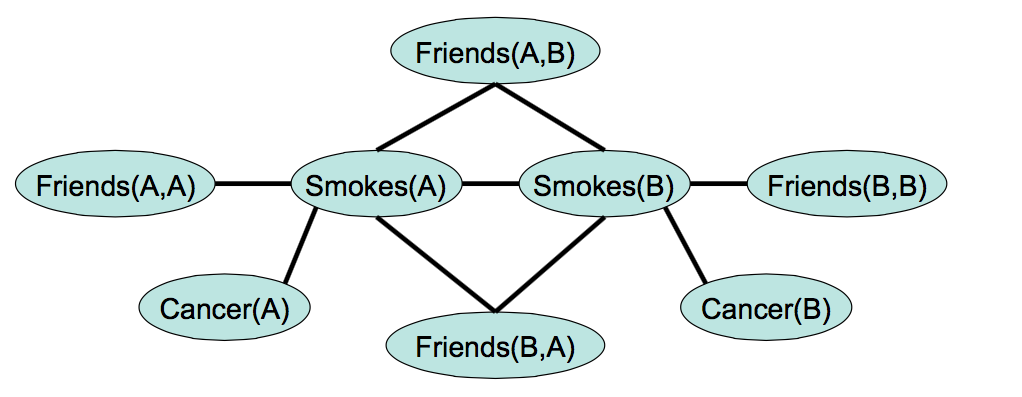
\includegraphics[scale=0.4]{mln}
  \caption{Beispiel}
\end{figure}

\mparagraph{Verbundswahrscheinlichkeit}
MLN ist eine Schablone für den Aufbau eines Markov Netzes. Die Wahrscheinlichkeit
einer Welt $X$ ist:
\begin{displaymath}
    P(X) = \frac{1}{Z}(\sum_{i}w_in_i(X))
\end{displaymath}
\begin{itemize}
    \item $w_i$: Gewicht der Formel $i$
    \item $n_i(X)$: Anzahl der wahren Belegung der Formeln $i$ in $X$.
\end{itemize}
Ein Beispiel für $n_i(X)$ könnte sein:
\begin{displaymath}
    n_i(X) = n_i(\text{smoking,cancer}) = \begin{cases}
                                                1, \text{ if} \neg\text{smoking}
                                                 \vee \text{cancer}\\
                                                0, \text{ otherwise}
                                        \end{cases}
\end{displaymath}

\mparagraph{Inferenz}
Mit MAP finden des wahrscheinlichsten Zustands der Welt (Variablen y,) gegeben Evidenzen
x (wahrscheinlichste Erklärung für y)

\begin{align}
    \argmax_y P(y | x) &= \frac{1}{Z} \exp(\sum_{i} w_i n_i(x, y))\\
         &= \sum_{i} w_i n_i(x, y)
     \end{align}

\chapter{Instanzbasiertes Lernen}

\mparagraph{Lazy Learning}
Beispiele werden einfach nur abgespeichert. Wenig Rechenzeit, doch mehr
Anfragen bei Klassifikation. Sollen neue Daten klassifiziert werden, so wird die
Klasse des ähnlichsten Datensatzes gewählt

\mparagraph{K-Nearest Neighbour}
Finde $k$ nächsten Nachbarn (euklidische Distanz) zum gesuchten $x_i$ und ordne
$x_i$ der Klasse der Mehrheit von den $k$ Nachbarn zu

\begin{displaymath}
f(x_i) \leftarrow \argmax_{v \in V} \sum_{i=1}^k \delta(v,c(x_i))
\end{displaymath}
\begin{equation}
    \delta(a,b) =
    \begin{cases}
        1, \text{ falls } a = b \\
        0, \text{ sonst}
    \end{cases}
\end{equation}

Bei gewichtetem k-NN wird $\delta(v,c(x_i))$ mit dem Gewicht $w_i$ multipliziert.
\begin{displaymath}
    w_i = \frac{1}{d(x_q,x_i)^2}
\end{displaymath}

\mparagraph{Case Base Reasoning}
Ist ans ich kein direkt anwendbarer Algorithmus. Die idee lautet, dass ähnliche,
bekannte Fälle gesucht werden welche auf den aktuellen Fall übertragen werden
können.
\begin{itemize}
    \item \textbf{Retrieve}: Finde ähnliche Fälle.
    \begin{itemize}
        \item Ähnlichkeitsmaß: Euklidische Distanz, Syntaktische Ähnlichkeit,
        Semantische Ähnlichkeit
        \item Organisation der Fallbasis: Lineare Liste, Baumstruktur, Graphen,
        Netze, Indexstrukturen, Datenbanken
    \end{itemize}
    \item \textbf{Reuse}: Lösungsadaption
    \item \textbf{Revise}: Überprüfung, Verbesserung der Lösung.
    \begin{itemize}
        \item Evaluierung der Lösung. Überprüfung durch Simulation/in der realen
        Welt
        \item Verbessern bzw. reparieren der Lösung. Fehler erkennen und erklären
        \item potentiell iterativ
    \end{itemize}
    \item \textbf{Retain}: Bewahrung der gemachten Erfahrung
\end{itemize}

Andwendung: CLAVIER, KogniMobil

\chapter{Deduktives Lernen}
Fakten werden gegeben. Der lernende bekommt das allgemeine Konzept gesagt und
 muss nur logische Schlussfolgerungen machen.

\mparagraph{Erklärungsbasiertes Lernen, EBL Explanation Based Learning}
The key insight behind explanation-based generalization
is that it is possible to form a justified generalization of a
single positive training example provided the learning
system is endowed with some \textbf{explanatory capabilities}. In
particular, the system must be able to explain to itself \textbf{why
the training example is an example of the concept} under
study. Thus, the generalizer is presumed to possess a
definition of the concept under study as well as domain
knowledge for constructing the required explanation.\\

Gegeben:
\begin{itemize}
    \item Zielkonzept: Beschreibung des zu lernenden Konzepts
    \item Trainigsbeispiel: Beispiel für das Zielkonzept
    \item Bereichstheorie: Regeln und Fakten, die erklären warum Trainigsbeispiel
    ein Beispiel für das Zielkonzept ist
    \item Operationalitäts-(Anwendbarkeits) Kriterium: Ein Prädikat über
    Konzeptbeschreibung, das die Form spezifiziert, in der erlernte Beschreibungen
    vorliegen müssen.
\end{itemize}

Gesucht:
\begin{itemize}
    \item Eine Generalisierung des Trainigsbeispiels, die eine hinreichende
    Definition des Zielkonzeptes darstellt und das Operationalitätskriterium erfüllt.

\end{itemize}
\mparagraph{Explanation Based Generalization, EBG}
Prozess, der implizites Wissen in explizites Wissen umwandelt. \\
EBG ist ein Zweischrittverfahren und geht wie folgt vor:
\begin{itemize}
    \item Explain: Finden einer Erklärung, die zeigt, warum das Trainigsbeispiel
    die Definition des Zielkonzeptes erfüllt $\rightarrow$ Modus Ponens anwenden.
    \item Generalize: Bestimme hinreichende Bedingungen, unter denen die oben
gefundene Erklärungsstruktur gültig ist und formuliere diese
Kriterien in Termen, die das Operationalitätskriterium erfüllen.
\end{itemize}
Bei EBG werden Makrooperatoren (Zusammengefasste Operatorsequenzen, welche die
Kosten für das Finden von Problemlösungswissen reduzieren) erzeugt.
STRIPS verwendet EGB.

\mparagraph{Deduktives vs. Induktives lernen}

\begin{table}[h!]
\centering

\begin{tabular}{|l|l|l|}
\hline
 & \textbf{Induktives Lernen} & \textbf{Deduktives Lernen} \\ \hline
\textbf{Ziel} & Hypothese passt du den Daten & Hypothese passt zur Bereichstheorie \\ \hline
\textbf{Vorteile} & wenig a-priori wissen & wenig Beispiele notwendig \\ \hline
\textbf{Nachteile} & \begin{tabular}[c]{@{}l@{}}- schlecht bei geringen Datenmengen\\ - schlecht bei inkorrektem Bias\end{tabular} & schlecht, falls imperfekte Bereichstheorie \\ \hline
\end{tabular}
\end{table}

\mparagraph{Lernproblem}
Seien $D$ Trainigsbeispiele, möglicherweise mit Fehlern, $B$ die Bereichstheorie,
möglicherweise Fehlerhaft und $H$ der Hypothesenraum. So lässt sich die
beste Hypothese $h$, welche am besten zu Trainigsbesiepiel als auch Bereichstheorie
passt mittels
\begin{displaymath}
    \argmin_{h \in H} k_D E_D(h) + k_bE_B(h)
\end{displaymath}
berechnen. Wobei
\begin{itemize}
    \item $E_D, E_B$: Fehlerrate bezüglich Trainigsdaten/Bereichstheorie
    \item $k_D, k_B$: relatives Gewicht für Trainigsdaten/Bereichstheorie
\end{itemize}

\mparagraph{Knowledge Based Artificial Neurol Network, KBANN}
KBANN ist ein hybrides Verfahren. Die Idee hierbei ist es mittels Bereichstheorie
ein Neuronales Netz zu initialisieren, welches durch Backpropagation und
Trainigsbeispiele verfeinert wird.

\begin{enumerate}
    \item Pro Instanzattribut wird ein Netz-Input verwendet. Für jede Klausel
    wird ein Neuron hinzugefügt
    \item Dieses ist mit dem Instanzattribut durch das Gewicht $w$ verbunden
    wenn es nicht negiert ist. Ansonsten $-w$
    \item Der Schwellwert wird auf $-(n-0.5)w$ gesetzt. $n$ ist die Anzahl der
    nicht negierten Bedingungsteile
    \item Verbinde die restlichen Neuronen von Schicht $i$ mit Schicht $i+1$ indem
    zufällige kleine Gewichte gesetzt werden.
\end{enumerate}

Anwendung:
\begin{itemize}
    \item Lernen von physikalischen Objektenklassen
    \item Erkennung biologischer Konzepte in DNS-Sequenzen
\end{itemize}

\chapter{Evolutionäre Algorithmen}

\mparagraph{Nomenklatur}
\begin{itemize}
    \item \textbf{Individuum}: eine mögliche Lösung, Hypothese
    \item \textbf{Population und Generation}: Lösung bzw. Hypothesenmenge
    \item \textbf{Erzeugen von Nachkommen}: Generierung neuer Hypothesen
    Methoden z.B \begin{itemize}
        \item Rekombination: Vermischen der Gene zweier Elternteile.
        \begin{itemize}
            \item diskret: ein Teil Gene von einem Elternteil
            übernommen werden und andere vom anderen Elternteil.
            \item intermediär: Nachkomme wird gemittelt $z_i = \frac{(x_i + y_i)}{2}$
            \item Crossover: aus 2 Eltern werden 2 Nachkommen. singlepoint,
            twopoint, uniform crossover.
        \end{itemize}
        \item Mutation: Veränderung einzelner Gene bei Abstammung von einem Elternteil.
        z.B
        \begin{itemize}
            \item Bitinversion: Feste anzahl aber zufällige Gene
            \item Translation: Verschieben einer Teilsequenz
            \item Invertiertes Einfügen
            \item spezielle Mutationsoperatoren sind andwendungsspezifisch.
        \end{itemize}
    \end{itemize}
    \item \textbf{Veränderter Nachfolger, Kind, Nachkomme}: neue Hypothese
    \item \textbf{Fitness Funktion}: Hypothesengüte, zu optimierendes Kriterium
    \item \textbf{Selektion der Besten}: Auswahl der Hypothesen, welche die
    beste Problemlösung erzeugen.
\end{itemize}

\mparagraph{Grundalgorithmus}
Solange fitness nicht optimal mache:
\begin{enumerate}
    \item Selektion der Eltern
    \item Generierung von Nachkommen
    \item Fitness bewertung
    \item Selektion der überlebenden Populationsmitglieder
\end{enumerate}

\mparagraph{Selektion}

Zwei arten der Selektion:
\begin{itemize}
    \item die Eltern für jeweilige Erzeugung von Nachkommen (mating)
    \item der Population für die nächste Iteration
\end{itemize}

Probleme:
\begin{itemize}
    \item \textbf{Genetische Drift}: Individuen vermehren sich zufällig mehr
    als andere. Diese sind nicht unbedingt besser für das Problem geeignet.
    \item \textbf{Crowding, Ausreißerproblem}: ''fitte'' Individuen und ähnliche
    Nachkommen dominieren die Population. Problematisch wegen lokaler Maxima.
\end{itemize}


\mparagraph{Mating}
Ist ein Populationsmodell
\begin{itemize}
    \item \textbf{Insellmodell}: lokal, die Evolution läuft weitgehend getrennt,
    nur manchmal werden Individuen ausgetauscht.
    \item \textbf{Nachbarschaftsmodell}: nahe Umgebung, Nachkommen dürfen nur von
    Individuen gezeugt werden, die in ihrere Nachbarschaft die beste Fitness
    besitzen.
    \item \textbf{Eine einfache Menge}: global, die global Besten entwickeln
    sich rasch weiter, andere Entwicklungslinien werden unterdrückt.
\end{itemize}

\mparagraph{Selektionsmethoden}

\begin{itemize}
    \item Fitness Based Selection \\
    $P(x) \approx \frac{\lambda}{\mu}\frac{f(x)}{\sum_{x' \in \text{Pop}} f(x')}$

    \begin{itemize}
        \item $P(x)$: Wahrschl. der Auswahl von Individuum $x$
        \item $\lambda$ Anzahl von Nachkommen
        \item $\mu$ Populationsgröße
        \item $f$ Fitness Funktion
    \end{itemize}
    \item Ranking Based Selection \\
    $P(x) \approx \frac{g(r(x))}{\sum_{x' \in \text{Pop}} g(r(x'))}$

    \begin{itemize}
        \item $P(x)$: Wahrschl. der Auswahl von Individuum $x$
        \item $r(x)$ ranking von x in der aktuellen Population gemäß Fitness
        Funktion
        \item $g$ Mit der Güte des Ranges monoton steigende Funktion
    \end{itemize}
    \item Tournament Selection
\end{itemize}

\mparagraph{Evolution}
\begin{itemize}
    \item \textbf{Lamarksche Evolution}: Individuen ändern sich (lernen) nach
    der Erzeugung. Genotyp (alle Gene) wird verändert und anschließend vererbt.
    \item \textbf{Baldwinsche Evolution}: Individuen ändern sich (lernen) nach
    der Erzeugung. Genotyp bleibt unverändert
    \item \textbf{Hybride Verfahren}: Es gibt veränderbare und fixe Phänotypen.
\end{itemize}

\mparagraph{Anwendungsbeispiele}
\begin{itemize}
    \item Travelling Salesman
    \item Flugplanoptimierung
    \item Mischung von Kaffeesorten
    \item Cybermotte: Motte müssen optimales Muster finden, um sich vor einer
    Fläche weißem Rauschen zu verbergen
    \item Optimale Steuerung in der Robotik
    \item Optimierung der Topologie Neuronaler Netze
    \item Optimierung des Muskel-Skelett Systems hinsichtlich energieeffizienter
Steuerung


\end{itemize}

\chapter{Einordnungskriterien}

% Please add the following required packages to your document preamble:
% \usepackage{multirow}
\begin{table}[h!]
\centering
\advance\leftskip-1.0cm
\scalebox{0.8}{
\begin{tabular}{|l|c|c|c|c|c|c|c|c|c|c|c|c|c|}
\hline
\multicolumn{2}{|c|}{\multirow{2}{*}{\textbf{Algorithmus}}} & \multicolumn{2}{c|}{\textbf{Inferenztyp}} & \multicolumn{2}{c|}{\textbf{Lernebene}} & \multicolumn{2}{c|}{\textbf{Lernvorgang}} & \multicolumn{2}{c|}{\textbf{Beispielumgebung}} & \multicolumn{2}{c|}{\textbf{Beispielumfang}} & \multicolumn{2}{c|}{\textbf{Hintergrundwissen}} \\
\multicolumn{2}{|c|}{} & ind. & ded. & symb. & subsymb. & überwacht & unüb. & inkr. & nicht inkr. & umfangreich & gering & emp. & axiom. \\ \hline
\multicolumn{2}{|l|}{Version space} & x &  & x &  & x &  & x &  & x &  & x &  \\ \hline
\multirow{2}{*}{NN} & klassisch & x &  &  & x & x &  & x &  & x &  & x &  \\ \cline{2-14}
 & \begin{tabular}[c]{@{}c@{}}auto-\\ encoder\end{tabular} & x &  &  & x &  & x &  & x & x &  & x &  \\ \hline
\multicolumn{2}{|l|}{Support Vector Machine} & x &  &  & x & x &  &  & x & x &  & x &  \\ \hline
\multicolumn{2}{|l|}{k-means clustering} & x &  &  & x &  & x &  & x & x &  & x &  \\ \hline
\multicolumn{2}{|l|}{AHC} & x &  &  & x &  & x &  & x & x &  & x &  \\ \hline
\multicolumn{2}{|l|}{COBWEB} & x &  & x &  &  & x & x &  &  & x & x &  \\ \hline
\multicolumn{2}{|l|}{Bayessche Netze} & x &  &  & x & x &  &  & x & x &  & x &  \\ \hline
\multirow{2}{*}{\begin{tabular}[c]{@{}l@{}}Decision\\ Tree\end{tabular}} & \begin{tabular}[c]{@{}c@{}}ID3/C4.5\\ Random Forest\end{tabular} & x &  & x &  & x &  &  & x & x &  & x &  \\ \cline{2-14}
 & ID5R & x &  & x &  & x &  & x &  & x &  & x &  \\ \hline
\multicolumn{2}{|l|}{Hidden Markov Machine} & x &  &  & x & x &  &  & x & x &  & x &  \\ \hline
\multicolumn{2}{|l|}{k-Nearest Neighbour} & x &  &  & x & x &  &  & x & x &  & x &  \\ \hline
\multicolumn{2}{|l|}{Case Base Reasoning} & x &  & x &  & x &  & x &  &  & x & x &  \\ \hline
\multicolumn{2}{|l|}{EBL} &  & x & x &  & x &  & x &  &  & x &  & x \\ \hline
\end{tabular}}
\end{table}



\end{document}
